\documentclass[12pt,a4paper,titlepage]{scrreprt}
\usepackage[utf8]{inputenc}
\usepackage[english]{babel}

\usepackage[backend=biber,style=alphabetic]{biblatex}

\usepackage{url}
\usepackage{hyperref}
\usepackage{fancyvrb}
\usepackage{csquotes}
\usepackage{upquote}
\usepackage{../lib/diagrams}

\usepackage{amsmath}
\usepackage{amssymb}
\usepackage{amsthm}
\usepackage{tikz}
\usetikzlibrary{matrix}

\newcommand{\catx}[1]{\mathbb{#1}}
\newcommand{\catC}{\catx{C}}
\newcommand{\catD}{\catx{D}}

\newcommand{\opcat}[1]{{#1}^{\text{op}}}
\newcommand{\Sets}{\mathbf{Sets}}
\newcommand{\Cat}{\mathbf{Cat}}
\newcommand{\Hask}{\mathbf{Hask}}

%% @TODO: invent some kid of inline 'code' style for this
\newcommand{\firstArr}{\texttt{first}}

%% @TODO: pick a 'math' style for arrow operations
\newcommand{\arrM}{\text{arr}}
\newcommand{\firstM}{\text{first}}
%% >>>, <<< are \ggg and \lll

\DefineVerbatimEnvironment{code}{Verbatim}{fontsize=\small,commandchars=\\\{\},codes={\catcode`$=3\catcode`_=8}}

\hypersetup{
    colorlinks,
    linkcolor=black,
    citecolor=black,
    filecolor=black,
    urlcolor=black
}


\theoremstyle{definition}
\newtheorem{proposition}{Proposition}
\newtheorem{definition}{Definition}
\newtheorem{example}{Example}

\theoremstyle{plain}
\newtheorem{lemma}{Lemma}
\newtheorem{theorem}{Theorem}

\renewcommand{\labelitemi}{$-$}

\bibliography{literature}

\title{Cat-arrows}
\author{%
    Johannes Emerich
        (\href{mailto:Johannes@emerich.de}{johannes@emerich.de})\\
    Ignas Vyšniauskas
        (\href{mailto:i.vysniauskas@gmail.com}{i.vysniauskas@gmail.com})
}
\date{}

\begin{document}


\maketitle

\begin{abstract}
    This is a report on Arrows.
\end{abstract}

\section{Context}
\begin{frame}
\frametitle{Liberating Programming from the ``von Neumann'' style}

\begin{itemize}
    \item John Backus' call for new language paradigm (1978)
    \begin{itemize}
        \item \emph{Functional} programming (``FP'') as combinatorial
              approach to program construction
        \item Construct programs in an algebra of programs
        \item Variables range over \emph{programs}, operations are \emph{on}
              programs (\emph{pointfree} style)
        \item Functional style: only one state transition per operation
    \end{itemize}
    \item Haskell as most popular language true to Backus' ideas
\end{itemize}
\end{frame}

\begin{frame}
\frametitle{Haskell is non-strict}

\begin{columns}[c]
    \begin{column}{.6\textwidth}
        \begin{itemize}
            \item Problem of functions in computing: non-termination
            \item \emph{Lift} all types by adding an \texttt{undefined} ($\bot$) bottom
                  element, lowest in information order
            \item Set $B = \{\textrm{True}, \textrm{False}\}$ lifted to $B_\bot
                  = B \cup \{\bot\}$
            \item Functions are $B_\bot \to B_\bot$
        \end{itemize}
    \end{column}
    \begin{column}{.4\textwidth}
        \begin{center}
        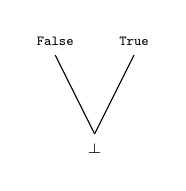
\begin{tikzpicture}
            \draw[font=\tiny] (0,0) node[below] {$\bot$} -- (0.5,1) node[above] {\texttt{True}};
            \draw[font=\tiny] (0,0) -- (-0.5,1) node[above] {\texttt{False}};
        \end{tikzpicture}
        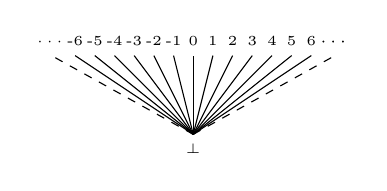
\begin{tikzpicture}
            \draw[dashed, font=\tiny] (0,0) -- (1.8,1) node[above] {$\cdots$};
            \draw[font=\tiny] (1.8,1) node[above] {$\cdots$};
            \draw[font=\tiny] (0,0) -- (1.5,1) node[above] {6};
            \draw[font=\tiny] (0,0) -- (1.25,1) node[above] {5};
            \draw[font=\tiny] (0,0) -- (1.0,1) node[above] {4};
            \draw[font=\tiny] (0,0) -- (0.75,1) node[above] {3};
            \draw[font=\tiny] (0,0) -- (0.5,1) node[above] {2};
            \draw[font=\tiny] (0,0) -- (0.25,1) node[above] {1};
            \draw[font=\tiny] (0,0) node[below] {$\bot$} -- (0,1) node[above] {0};
            \draw[font=\tiny] (0,0) -- (-0.25,1) node[above] {-1};
            \draw[font=\tiny] (0,0) -- (-0.5,1) node[above] {-2};
            \draw[font=\tiny] (0,0) -- (-0.75,1) node[above] {-3};
            \draw[font=\tiny] (0,0) -- (-1,1) node[above] {-4};
            \draw[font=\tiny] (0,0) -- (-1.25,1) node[above] {-5};
            \draw[font=\tiny] (0,0) -- (-1.5,1) node[above] {-6};
            \draw[dashed, font=\tiny] (0,0) -- (-1.8,1) node[above] {$\cdots$};
        \end{tikzpicture}
        \end{center}
    \end{column}
\end{columns}
\end{frame}

\begin{frame}[fragile]
\frametitle{Haskell is non-strict}
\begin{itemize}
    \item \emph{Strict} semantics
          \[
            \forall f: A_\bot \to B_\bot, f(\bot) = \bot
          \]
    \item Non-strict semantics allow operating on (potentially) infinite data
          structures:
          \begin{center}\verb|or ([True] ++ repeat False) == True|\end{center}
    \item Expressions only partially evaluated (\emph{thunks}) until value needed
    \item Problem for effectful computations whose result is never
          needed, e.g.
          \begin{center}\verb|print "Hello, Dave!"|\end{center}
\end{itemize}
\end{frame}

\begin{frame}[fragile]
\frametitle{Haskell is pure}
\begin{itemize}
    \item Functions are mappings from domain to codomain
    \item Haskell functions are \emph{pure}, they are \emph{only} mappings
    \item No side-effects (input/output, changes to global state)
    \item Beneficial for achieving Backus' desiderata
    \item But side-effects are desirable feature of programs
    \item How to bring them back in?
\end{itemize}
\end{frame}

\begin{frame}[fragile]
\frametitle{Computational lambda-calculus and monads}
\begin{itemize}
    \item Eugenio Moggi ('89): program equivalence in $\lambda$-calculus
    \item Semantics for \emph{general} notion of computation
          \begin{itemize}
              \item Side-effects, non-determinism, non-termination
          \end{itemize}
    \item Categorical language semantics with types as objects
          \begin{itemize}
              \item Distinguish type $B$ from corresponding \emph{computations} $TB$
              \item Model each notion of computation as a monad
          \end{itemize}
    \item Adopted into Haskell as general interface to computation
          \begin{itemize}
              \item Functions have to be pure, computations don't
          \end{itemize}
\end{itemize}
\end{frame}

\chapter{Modelling Computation in Theory and Practice}
    \section{Arrows in Haskell}

If all that computer programs do would be to operate on a fixed number of inputs
to produce output at most one time (that is, to never halt or terminate with
the result), pure language semantics would be sufficient. But real programs do
much more than that. They are interactive, that is, they query the environment
for input during runtime, and depend on this additional input for their runtime
behavior. They cause effects in their environment by leveraging built-in
capabilities of the machine they run on. They may run indefinitely, all the
while periodically producing output.

All of these types of computation are impossible to achieve with a pure
language, so any general purpose programming language needs to have notions of
computation to capture all of the above, and more.

In Haskell, the most obvious type of a computation with input of type \verb|a|
and output of type \verb|b| is the pure function type \verb|a -> b|, which is
built from types \verb|a| and \verb|b| by the \verb|(->)| type constructor. It
seems to make sense to adopt this notion of a computation being from something
to something\footnote{We could always make it from or to some uninteresting
fixed thing if we don't care about parameters or output.}, so we will generally
expect any type of computation to be a two-parametric type.

One of the powerful features of Haskell is the possibility of treating functions
as values, empowering programmers to build up complex functionality from simple
functions by assembling them using \emph{function combinators}. It seems
sensible, though not necessary, to expect equivalent compositionality for other
types of computation. The most basic kind of combinator for functions is
composition, and we will require an analogue. Our common expectations for types
of computations can be expressed in Haskell using a \emph{type class}.

\begin{code}
  class Computation a where
      (>>>) :: a b c -> a c d -> a b d
\end{code}

This in essence states that any type \verb|a| can be made a computation by
giving an implementation of the ``composition'' function, \verb|(>>>)|,
combining two computations \verb|a b c| and \verb|a c d| to a computation
\verb|a b d|.

Under these preconditions it seems clear that any pure function should always
fulfill the requirements for any kind of computation, so we require additionally
an embedding of pure functions into computation types, arriving at type class

\begin{code}
  class Computation a where
      pure   :: (b -> c) -> a b c
      (>>>)  :: a b c -> a c d -> a b d\textrm{.}
\end{code}

It should become clear from the act of choosing common requirements for
computations that this is not the only possible interface. And in fact,
historically, it was not the first approach implemented in Haskell. As sketched
in the introduction, the related but similar notion of monads was adopted from
category theory with requirements described by something akin to

\begin{code}
  class Monad m where
      return :: a -> m a
      fmap   :: (a -> b) -> m a -> m b
      (>>=)  :: m a -> (a -> m b) -> m b\textrm{,}
\end{code}

with \verb|return| describing how to turn values of type \verb|a| into
computations of type \verb|m a|, \verb|fmap| explaining how \verb|m| is an
endofunctor on the category of types, and \verb|(>>=)| a combinator for monads
and Kleisli arrows. With this model of computation, it is possible to model
computations with a specific return type, but without regard to specifically
\emph{structured} input of the computation.

While this is convenient in many cases, the method of producing computations of
type \verb|m b| from values of type \verb|a| by means of function application
dooms the combinator \verb|(>>=)| to execute computation \verb|m a| before being
able to actually construct a computation \verb|m b|. This sequencing means that
it is impossible for the \verb|(>>=)| combinator to analyse commonalities in
the input structure. Unfortunately, this property of the monad structure entails
that certain optimisations are out of bounds.

This is disappointing, as it limits the practicability of the monad as a general
interface to computation. By the time this detriment became clear, illustrated
in the work on LL(1) parsers by Swierstra and Duponcheel (\cite{swierstra}), the
benefits of such a general interface had become clear however. This incited John
Hughes's proposal of a notion of computation along the lines of above's
\verb|Computation|, which he called \emph{arrows}\footnote{Why this name? The
authors could not find an explanation in the literature, but as each kind of
\emph{arrow} in Hughes's sense describes the arrows---that is, morphisms---in
some category of data types, this seems like a likely reason.}.

The \verb|Arrow| typeclass proposed in~\cite{hughes-monad2arr} contains one
additional request atop \linebreak\verb|Computation|, as this is actually
\emph{too} general. We can observe that its applicability is seriously
diminished by the fact it gives no general way of combining the \emph{results}
of computations. A concise way of enabling this kind of operation is the
addition of the function \verb|first|:

\begin{code}
  class Arrow a where
      arr   :: (b -> c) -> a b c
      (>>>) :: a b c -> a c d -> a b d
      first :: a b c -> a (b, d) (c, d)
\end{code}

This interface allows the definition of a kind of non-commutative product with
signature,

\begin{code}
  (***) :: Arrow a => a b c -> a b' c' -> a (b, b') (c, c')\textrm{.}
\end{code}

In addition to the constraints expressed by the type class, the semantics of the
functions are subject to a set of laws, the \emph{arrow laws}, which need to be
verified by the author of each instance's implementation.

\begin{code}[numbers=left]
                (a >>> b) >>> c == a >>> (b >>> c)
                    arr (g . f) == arr f >>> arr g
                   arr id >>> a == a
                              a == a >>> arr id
            first a >>> arr fst == arr fst >>> a
     first a >>> arr (id *** f) == arr (id *** f) >>> first a
  first (first a) >>> arr assoc == arr assoc >>> first a
                  first (arr f) == arr (f *** id)
                first (a >>> b) == first a >>> first b
\end{code}

Note that \verb|(***)| as used in the laws is the product on \emph{pure}
functions. The function \verb|assoc| translates tuples \verb|((a,b),c)| to
\verb|(a,(b,c))|, and the functions \verb|fst| and \verb|snd| produce the first
and second position of a tuple, respectively.

The obvious instance of \verb|Arrow| is the pure function type \verb|(->)|. With
\verb|(.)| being the composition function for pure functions, functions of the
adequate types can be given by

\begin{code}
  instance Arrow (->) where
      arr f     = f
      (>>>) f g = (.) g f
      first f   = \symbol{92}(x, y) -> (f x, y)\textrm{,}
\end{code}

where the right-hand expression in the definition of \verb|first| is an
anonymous function defined on pairs \verb|(x, y)|.

% TODO Example of an actual NON-pure computation?

    \section{Freyd categories}

Freyd-categories were introduced by Power \& Robinson~\cite{pow-rob} as a type
of symmetric premonoidal category where the monoidal structure is given by
(the usual) \emph{product} operation. In the paper, this is merely a specific
case of the general notion of symmetric premonoidal categories, which are
proposed as generalisations of monoidal categories for modelling
non-commutative computational effects, such as non-determinism, exceptions and
concurrency.

The actual name, \emph{Freyd-}, is given in a later paper by Power \&
Thielecke~\cite{pow-thie} where Freyd-categories are examined as generalisations
of Cartesian closed categories and closed Freyd-categories are shown to be
models of Moggi's computational $\lambda$-calculus.

It is important to note that, in particular, Power \& Robinson showed that
Freyd-categories generalise strong monads, which were proposed by
Moggi~\cite{moggi-89} as categorical constructs for modelling effectful
computation. Hence the claimed computational-notion generalisations are
directly proved via category theory.

We shall now introduce the necessary notions to describe Freyd-categories and
some basic results about them.

\begin{definition}[Binoidal category]
    A binoidal category is a category $\catC$ equipped with:
    \begin{enumerate}
        \item for each $(A, B)$ in $|\catC| \times |\catC|$, an object $A \otimes B$
            in $|\catC|$;
        \item for each $A$, a functor $(A \rtimes -) : B \mapsto A \otimes B$
        \item for each $A$, a functor $(- \ltimes A) : B \mapsto B \otimes A$
    \end{enumerate}
\end{definition}

The conditions imply that, $A \rtimes B = A \otimes B = A \ltimes B$,
justifying the usage of the notation $A \otimes B$. Observe that this
operation is defined only on objects of $\catC$ so far.

\begin{definition}[Central morphism]
    A morphism $f: A \to B$ in a binoidal category is \emph{central} if for
    every morphism $g: A' \to B'$ the composites of maps (of the form $h
    \ltimes C$ or $C \rtimes h$, where $C$ is either $A$ or $B$ and $h$ is
    either $f$ or $g$) from $A \otimes A'$ to $B \otimes B'$ and from $A'
    \otimes A$ to $B' \otimes B$ agree.
\end{definition}

A natural transformation is central if its components are central.

Having these, we can now define the generalisation of monoidal category.

\begin{definition}[Premonoidal category]
    A \emph{premonoidal category} is a binoidal category equipped with:
    \begin{enumerate}
        \item an \emph{identity object} $I$
        \item for all $A, B, C$, a natural central \emph{associator}
            isomorphism $\alpha_{A,B,C}\colon (A \otimes B) \otimes C \to A
            \otimes (B \otimes C)$
        \item for each object $A$, natural central isomorphisms: \emph{left
            unitor} $\lambda_A\colon A \otimes I \to A$ and \emph{right unitor}
            $\rho_A\colon I \otimes A \to A$
    \end{enumerate}

    such that the usual monoidal category coherence conditions are satisfied,
    i.e.~the pentagon law for $\alpha$ and triangle laws for $\alpha$,
    $\lambda$, $\rho$ hold.

\end{definition}

\begin{example}[Described in \cite{gen-comp-eff-models}]
    Let $\catC$ be a category with finite products and $S$ a specified object
    in $\catC$ (which we regard as \emph{state} or \emph{context}).

    Define $\catx{K}$ as a category such that $|\catx{K}| := |\catC|$ and
    $\catx{K}(X, Y) := \catC(S \times X, S \times Y)$, with composition in
    $\catx{K}$ determined by the composition in $\catC$.

    For any object $X$ of $\catC$, one has evident functors
    $X \otimes -: \catx{K} \to \catx{K}$ and
    $- \otimes X: \catx{K} \to \catx{K}$ extending the product in $\catC$.

    The maps are not bifunctorial (with respect to $\otimes$), hence do not
    yield a monoidal structure on $\catx{K}$. However, they do  yield a
    premonoidal structure on $\catx{K}$.
\end{example}
%% @TODO: grok this example and explain it more.

A \emph{strict premonoidal category} is a premonoidal category in which all the
isomorphisms described above are identities, the $\otimes$ operator is
associative on objects and moreover $I$ is really an identity for $\otimes$.

Note that a strict premonoidal category need not be a monoidal one.

A \emph{symmetric premonoidal category} is a premonoidal category equipped with
a central natural isomorphism $\gamma_{A,B} : A\otimes B \cong B\otimes A$, with
the usual coherence conditions of symmetric monoidal categories.

The \emph{centre} of a premonoidal category $\catC$ is a subcategory $\catC'$,
such that $|\catC| = |\catC'|$ and all the morphisms in $\catC'$ are central.

The centre of a premonoidal category is a monoidal
category~\cite[Prop.~3.1]{pow-rob}.
Hence, a monoidal category is simply a premonoidal category in which all
morphisms are central.

A \emph{strict} (resp. \emph{symmetric}) \emph{premonoidal functor} is a functor which
preserves the strict (resp. symmetric) premonoidal structure and sends central
maps to central maps.

We can now define Freyd categories.

\begin{definition}[Freyd category]
    A Freyd category consists of a category with finite products $\catC$
    and an identity-on-objects strict symmetric premonoidal functor
    \[ J: \catC \to \catx{K} \]
    (hence $\catx{K}$ is a symmetric premonoidal category).
\end{definition}

The definitions of premonoidal categories, and especially Freyd categories,
might seem a bit involved at first sight, however they arise as quite
reasonable generalisations of monoidal categories when one deals with
computational effects. It is hard to phrase this better than one of the
``discoverers'' of Freyd categories, John Power~\cite{gen-comp-eff-models}:

%% @TODO: shorten this and maybe come-up with own motivation / examples
%% if there's time.
\begin{quote}
    The notion of Freyd-category has emerged over the past 15 years as a subtle
    generalisation of the notion of category with finite products. It allows
    one to model environments in call-by-value programming languages containing
    computational effects, notably the $\lambda_c$-calculus, a variant of the
    call-by-value $\lambda$-calculus designed specifically to allow one to account
    for computational effects. Starting with the notion of category with finite
    products, one obtains the notion of a symmetric monoidal category by
    dropping insistence upon the existence of diagonals and projections: in
    such situations, one usually speaks of a tensor product rather than a
    product, corresponding to the relaxation from cartesian logic to linear
    logic. If one further drops the insistence upon bifunctoriality of the
    tensor product, one obtains the notion of a symmetric premonoidal category.
    This corresponds logically to keeping the terms of linear logic but putting
    fewer of them equal.  Just as one has cartesian closed categories and
    symmetric monoidal closed categories, one can speak of closedness for a
    symmetric premonoidal category too. Finally, if one reinstates the
    assumption of finite product structure but only on a specified subcategory
    of a putative symmetric premonoidal category, one has the notions of
    Freyd-category and closed Freyd-category [\ldots]
\end{quote}

\chapter{Categorical semantics of arrows (?)}
    \section{A short history of the categorical aspects of arrows}
\label{sec:cat-arrows-hist}

Unlike Monads, which were borrowed from category theory to model various
computational behaviours, arrows were at first introduced by
Hughes~\cite{hughes-monad2arr} purely as a computational concept. Hence
categorical \emph{interpretations} of arrows came only as an afterthought.
Unsurprisingly, a whole family of interpretations was thus born, which we try
to describe briefly here. % and possibly expand on it later on

The tale of the categorical semantics of arrows begins with a folklore
statement
\begin{displayquote}Arrows are Freyd categories.\end{displayquote}
%% wtf -- this quoting is ugly -- want emph + quotemarks @TODO: fix
which is perhaps first noted by Paterson~\cite{paterson}.

This statement was first verified in detail by Heunen and
Jacobs~\cite{arr-like-mon}. Since computationally arrows are a generalisation
of monads, it is perhaps not so surprising that the situation turns out to be
similar categorically. Namely, Heunen and Jacobs prove that arrows can be
seen as monoids in categories of bifunctors $\opcat{\catC} \times \catC \to
\catC$, just like monads are monoids in a category of endofunctors.
Furthermore, they show there is a bijective correspondence between locally
small Freyd categories $\catC \to \catD$ and arrows over $\catC$.

However, the construction is slightly flawed due to issues with the size of
$\catC$.\footnote{$\catC$ would need to be both small and (co)complete, however
this is impossible~\cite[Chapter 3]{freyd-abelian-cats}} %% @TODO: insert citation
Hence, the statement \enquote{Arrows are Freyd} is only proved for bifunctors
on $\opcat{\catC} \times \catC \to \Sets$, where $\catC$ is \emph{small} (i.e.\ 
profunctors) with an assumption that it would be possible to achieve the same
result in an enriched setting.

A later paper by Hasuo and Jacobs called ``Freyd is Kleisli, for
Arrows''~\cite{freyd-is-kleisli} elaborates on the fact that the correspondence
is actually an instance of the well-known Kleisli construction for monads,
adapted for arrows. This again goes along with the general intuition that
arrows are a generalisation of monads.

%% @TODO: I'm not sure whether my interpretation of this is fully correct.
%% In particular, I need to check whether they are just examining the same
%% correspondance, or building something new.
%% They seem to be talking about a 'monoidal' interpretation and a Freyd one,
%% as of two different things...
%% Perhaps it's best to re-iterate this statement after we write-up the
%% 'meat' parts.

Another paper by Jacobs, Heunen and Hasuo~\cite{cat-semantics-arr} combines the
previous results into a self-contained paper and will be our primary reference.

Finally, a paper by Atkey~\cite{atkey-fix} notes that the work of Jacobs et.~al
slightly misinterprets the situation. Firstly, Atkey elaborates on the fact
that it is necessary to consider enriched Freyd categories, because in order to
provide denotational semantics for arrows one needs to consider a \emph{type}
of morphisms between objects (which are types too), hence one needs at least
some sort of self-enrichment. More importantly, Atkey observes that the
\firstArr{} operator allows arrows to take \emph{unstructured} input. This does
not fit-in with the simplified ``Arrows are Freyd'' view, because it implies
that all computations are structured, which prevents modelling unstructured
input. Atkey thus shows that one also needs to consider indexed Freyd categories and
proves various relations between \{closed, indexed, enriched\} Freyd categories,
arrows and strong monads.

    \section{Arrows are monoids}

%% Disclaimer: I allowed myself to freestyle here, so please read with
%% suspicion.

We now explore a rather simplified interpretation of arrows, mostly following
the one initially described by Heunen \& Jacobs~\cite{arr-like-mon}. Our spirit
here is to just assume that the naive categorical interpretations of arrow
definitions are correct and then see what structure this gives us.
Using this approach we end up with the fact that arrows can be seen as monoids
on the category of bifunctors $\opcat{\catC} \times \catC \to \catC$.
Moreover, we also obtain a (sloppy) bijection between Freyd categories and
the aforementioned monoidal structure induced by arrows.

Since arrows are first of all a computational notion in functional programming,
to begin, we can, as usual, assume our working domain is some cartesian closed
category $\catC$. In particular, we can consider $\catC$ to be the category
$\Hask$ of Haskell types and functions.

Having this domain in mind, we can try to provide a categorical interpretation
of a Haskell \verb|(Arrow a)| instance. First, observe that every type
constructor \verb|f :: * -> *| in Haskell induces a subcategory of $\Hask$
where all types (i.e.~objects) are of the form \verb|f a|.  Similarly,
the \verb|(Arrow a)| type constructor \verb|a| of kind \verb|* -> (* -> *)|
also induces a subcategory of function types.\footnote{%
For intuition, observe that e.g. the function type constructor
\texttt{(->)} is of kind \texttt{* -> (* -> *)}}
%% can't use \verb in footnote for mysterious reasons

With these observations, we can deduce that it is reasonable to consider
\verb|(Arrow a)| categorically as, firstly, a map $A$, whose object part is
of the form $|\catC| \to |\catC \Rightarrow \catC|$, which after uncurrying
becomes $|A|: |\catC| \times |\catC| \to |\catC|$. Moreover, since we want $A$
to play nice with Haskell functions, we assume it is well-behaved with respect
to morphisms in $\Hask$, which boils down to $A$ being bifunctorial.

Moreover, we see $A$ is contravariant in the first variable and covariant in
the second. Thus we can conclude that $A$ is in fact an endo-profunctor on
$\catC$, i.e.~$A: \opcat{\catC} \times \catC \to \catC$. We later prove our
assumptions are correct\footnote{By which we mean: ``correct for the naive
interpretation''} and now consider the additional structure induced by
the arrow operations:

\begin{itemize}
    \item \verb|arr| is a function of type \verb|(b -> c) -> a b c|.
        The categorical interpretation of a function type is simply an internal
        hom in $\catC$, hence we get that categorically \verb|arr| corresponds
        to a functor sending homs in $\catC$ to homs in the subcategory induced
        by $A$, i.e.: $arr: [B \Rightarrow C] \mapsto A(B, C)$. Alternatively, one
        can say that $arr$ is a collection of natural transformations
        $arr_{BC}$, sending morphisms $B \to C$ in $\catC$ to morphisms in $A$;
    \item similarly, \verb|first| is function of type
        \verb|a b c -> a (b, d) (c, d)|
        corresponding to a family of morphisms\\
        $first_{BCD}: A(B, C) \to A(B \times D,C \times D)$\\
        or as a functor $first$ sending homs $A(-, +)$ to homs $A(- \times D, +
        \times D)$;
    \item finally, \verb|(>>>)| is function of type \verb|a b c -> a c d -> a b d|.
        If $A$ were closed then, we could interpret \verb|(>>>)| as a
        map\\
        $\ggg_{BCD}: A(B, C) \to (A(C, D) \Rightarrow A(B, D))$.\\
        However, this is not the case in general, so instead we can view
        \verb|(>>>)| as a family of morphisms\\
        $\ggg_{BCD}: A(B, C) \times A(C, D) \to A(B, D)$\\
\end{itemize}

We assume for now that our interpretations are correct (in particular, that the
claimed natural transformations are actually natural) and move on to take a
closer look at $\ggg$.

\begin{lemma}[{\cite[Lemma~3.3]{arr-like-mon}}]
    The maps $\ggg: A(X, P) \times (P, Y) \to A(X, Y)$ are natural in $X$,
    $Y$ and dinatural in $P$.
\end{lemma}

Advanced category theory wizards upon spotting dinaturality take to looking
for a tensor structure~\cite[p.~8]{arr-like-mon}. Hence we shall try to follow
their path.

    \section{Arrows are Freyd categories}

Having gained some acquaintance with both Freyd categories as well as arrows and
their categorical interpretation, we now return to the \emph{folklore} claim
encountered in~\ref{sec:cat-arrows-hist}. We will follow the exposition
in~\cite{cat-semantics-arr} to give a formal meaning to the claim. To do so, we
will first give a way of constructing categories from arrows such that they give
rise to Freyd categories. Second, we will complete the correspondence by showing
how Freyd categories give rise to arrows.

Before however getting into the meat of this section, we want to summarize the
results of this chapter in so far in

\begin{definition}[Arrows categorically]\label{def:catarr}
    Let $\catC$ be a locally small category with finite products. Define an
    \emph{arrow over $\catC$} to be a monoid in the category of profunctors
    $\opcat{\catC} \times \catC \to \catC$ possessing a natural transformation
    $first$, whose components $first_Z: A(X, Y) \to A(X \times Z, Y \times Z)$
    satisfy the arrow laws (5)--(9).
\end{definition}

Now for the new part.

\begin{definition}
    For an arrow $A : \opcat{\catC} \times \catC \to \catC$ with operations
    $arr, \ggg$, and $first$, define $\catC_A$ by
    \begin{itemize}
        \item $|\catC_A| := |\catC|,$
        \item $\catC_A(X, Y) := A(X, Y),$
        % TODO Mark respective cats?
        \item for $X \in \catC_A$, $1_X := arr(id_X),$
        \item for $f: X \to Y, g: Y \to Z, g \circ f := f \ggg g$.
    \end{itemize}
\end{definition}

\begin{proposition}
    $J_A : \catC \to \catC_A, X \mapsto X, f \mapsto arr(f)$ is a functor.
\end{proposition}

\begin{proof}
    This follows from the definition of $\catC_A$ and the arrow laws, whereby
    $J_A(g \circ f) = arr(g \circ f) = arr(f) \ggg arr(g) = g \circ_{\catC_A}
    f$.
\end{proof}

We shall now show that this gives rise to a Freyd category.

\begin{lemma}
    For an arrow $A : \opcat{\catC} \times \catC \to \catC$ over a category
    $\catC$ with finite products, the category $\catC_A$, together with $\catC$
    and $J_A : \catC \to \catC_A$ forms a Freyd category.
\end{lemma}

% The proof, the proof, the proof is on fire.
\begin{proof}
    To see that $\catC_A$ is symmetric premonoidal, take $I$ to be the initial
    object of $\catC_A$ and define $\alpha_{X, Y, Z}^{\catC_A} := arr(\alpha_{X,
    Y, Z}), \lambda^{\catC_A}_X := arr(\lambda_X), \rho^{\catC_A}_X :=
    arr(\rho_X),$ and $\gamma^{\catC_A}_{X, Y} := arr(\gamma_{X, Y})$. The
    operation $X \otimes Y := X \times Y$ can be extended to a functor by
    setting, for $f: X \to Y$, $f \ltimes Z := first_Z(f)$, and $Z \rtimes f :=
    second_Z(f)$.
    % TODO Does this suffice to show $\catC_A$ is premonoidal?

    Since $J_A$ is the identity on objects and $arr$ on morphisms, it only
    remains to show that it also preserves central maps. Let then $f: X \to X'$
    be some morphism from $\catC$ (hence it is central). We need to verify that
    $J_Af$ is central in $\catC_A$. Let for this $g : Y \to Y'$ be some
    arbitrary morphism from $\catC_A$, then we want
    \[
    \begin{diagram}
        X \otimes Y         & \rTo^{J_Af \ltimes Y}  & X' \otimes Y \\
        \dTo^{X \rtimes g}  &                        & \dTo_{X' \rtimes g} \\
        X \otimes Y'        & \rTo^{J_Af \ltimes Y'} & X' \otimes Y'
    \end{diagram}
    \]
    to commute, which is just
    % TODO Introduce second
    \[
    \begin{diagram}
        X \otimes Y         & \rTo^{first_Y(arr(f))}    & X' \otimes Y \\
        \dTo^{second_X(g)}  &                           & \dTo_{second_{X'}(g)} \\
        X \otimes Y'        & \rTo^{first_{Y'}(arr(f))} & X' \otimes Y'
    \end{diagram}
    \]
    and follows from the arrow laws and the definition of $second$ by:
    \begin{align*}
        first_Y(arr(f)) \ggg second_{X'}(g)
          &= arr(f \times id_Y) \ggg second_{X'}(g) \\
          &= arr(f \times id_Y) \ggg arr(\gamma_{X'Y}) \ggg first_{X'}(g) \ggg arr(\gamma_{Y'X'}) \\
          &= arr((f \times id_Y) \circ \gamma_{X'Y}) \ggg first_{X'}(g) \ggg arr(\gamma_{Y'X'}) \\
          &= arr(\gamma_{XY} \circ (id_Y \times f)) \ggg first_{X'}(g) \ggg arr(\gamma_{Y'X'}) \\
          &= arr(\gamma_{XY}) \ggg arr(id_Y \times f) \ggg first_{X'}(g) \ggg arr(\gamma_{Y'X'}) \\
          &= arr(\gamma_{XY}) \ggg first_{X}(g) \ggg arr(id_{Y'} \times f) \ggg arr(\gamma_{Y'X'}) \\
          &= arr(\gamma_{XY}) \ggg first_{X}(g) \ggg arr((id_{Y'} \times f) \circ \gamma_{Y'X'}) \\
          &= arr(\gamma_{XY}) \ggg first_{X}(g) \ggg arr(\gamma_{Y'X} \circ (f \times id_{Y'})) \\
          &= arr(\gamma_{XY}) \ggg first_{X}(g) \ggg arr(\gamma_{Y'X}) \ggg arr(f \times id_{Y'}) \\
          &= arr(\gamma_{XY}) \ggg first_{X}(g) \ggg arr(\gamma_{Y'X}) \ggg first_{Y'}(arr(f)) \\
          &= second_X(g) \ggg first_{Y'}(arr(f)).
    \end{align*}
    For the other diagram,
    \[
    \begin{diagram}
        Y \otimes X        & \rTo^{Y \rtimes J_Af}  & Y \otimes X' \\
        \dTo^{g \ltimes X} &                        & \dTo_{g \ltimes X'} \\
        Y' \otimes X       & \rTo^{Y' \rtimes J_Af} & Y' \otimes X',
    \end{diagram}
    \]
    that is,
    \[
    \begin{diagram}
        Y \otimes X       & \rTo^{second_Y(arr(f))}    & Y \otimes X' \\
        \dTo^{first_X(g)} &                            & \dTo_{first_{X'}(g)} \\
        Y' \otimes X      & \rTo^{second_{Y'}(arr(f))} & Y' \otimes X',
    \end{diagram}
    \]
    the procedure is similar.
\end{proof}

\begin{lemma}
    Every Freyd category of the form $\catD, \catC, J: \catC \to \catD$ induces
    an arrow.
\end{lemma}

\begin{proof}
    Define $A: \opcat{\catC} \times \catC \to \catC$ by setting $A(X, Y) :=
    \catD(X,Y)$. We first need to verify that $A$ forms a monoid in the category
    of $\catC$-enriched profunctors $\opcat{\catC} \times \catC \to \catC$ with
    appropriate unit and multiplication.

    Let for this $arr(f) := Jf$ and $a \ggg b := b \circ_\catD a$. A quick
    verification of the arrow laws (1)--(4) can be done by noting that (1) is
    inherited from the composition of $\catD$, (2) holds since $J$ is a functor
    on $\catC$, and the same is true for (3) and (4).

    $first$ can be given as
    \[
        first_Z(a) := (arr(\lambda p : X \times Z. (p, p))
          \ggg ((arr(\pi_1) \ggg a) \ltimes X \times Z))
          \ggg arr(id_Y \times \pi_2).
    \]
    The checking of the arrow laws (5) through (9) for this definition is intricate
    and omitted\footnote{The proof in~\cite{cat-semantics-arr} uses the notion
    of \emph{internal strength} in place of $first$, which we avoid for
    terminological simplicity, but whereby this verification is complicated.}.
%    \begin{align*}
%        & first_Z(a) \ggg arr(\pi_1) \\
%        & \quad = \big(arr(\lambda p : X \times Z. (p, p))
%          \ggg ((arr(\pi_1) \ggg a) \ltimes X \times Z)\big)
%          \ggg arr(id_Y \times \pi_2) \ggg arr(\pi_1) \\
%        & \quad = \big(arr(\lambda p : X \times Z. (p, p))
%          \ggg ((arr(\pi_1) \ggg a) \ltimes X \times Z)\big)
%          \ggg arr(\pi_1 \circ (id_Y \times \pi_2)) \\
%        & \quad = \big(arr(\lambda p : X \times Z. (p, p))
%          \ggg ((arr(\pi_1) \ggg a) \ltimes X \times Z)\big)
%          \ggg arr(\pi_1) \\
%        & \quad = \big(arr(\lambda p : X \times Z. (p, p))
%          \ggg ((arr(\pi_1) \ltimes X \times Z) \ggg (a \ltimes X \times Z))\big)
%          \ggg arr(\pi_1) \\
%        & \quad \overset{(1)}{=} \big(arr(\lambda p : X \times Z. (p, p))
%          \ggg (arr(\pi_1) \ltimes X \times Z)\big)
%          \ggg \big((a \ltimes X \times Z) \ggg arr(\pi_1)\big) \\
%        & \quad = \big(arr(\lambda p : X \times Z. (p, p))
%          \ggg (arr(\pi_1) \ltimes X \times Z)\big)
%          \ggg a \\
%        & \quad = \big(arr(\lambda p : X \times Z. (p, p))
%          \ggg (arr(\pi_1) \ltimes X \times Z)\big)
%          \ggg a \\
%    \end{align*}
%    \begin{align*}
%        & first_Z(arr(f)) \\
%        & \quad = \big(arr(\lambda p : X \times Z. (p, p))
%                    \ggg ((arr(\pi_1) \ggg arr(f)) \ltimes X \times Z)
%                  \big)
%                  \ggg arr(id_Y \times \pi_2) \\
%        & \quad = \big(arr(\lambda p : X \times Z. (p, p))
%                    \ggg (arr(f \circ \pi_1) \ltimes X \times Z)
%                  \big)
%                  \ggg arr(id_Y \times \pi_2)
%    \end{align*}
\end{proof}
The two lemmas together establish the main result of~\cite{cat-semantics-arr}.
\begin{theorem}[``Arrows are Freyd categories'']
    Given any locally small category $\catC$ with finite products, there is a
    one-to-one correspondence between arrows $A$ over $\catC$ and locally small
    Freyd categories $\catC \to \catD$.
\end{theorem}


\nocite{mustard}
\printbibliography

\end{document}
